\chapter{Análise Bibliográfica sobre Neurociência e Inteligência Artificial por Stefano Luppi Spósito\label{chap:bibliometria:kawaiistheno}}

\section{Planejamento do Estudo}

Atualmente, é fato que o ser humano está sempre conectado à tecnologia de alguma forma, seja pelo seu smartphone ou pelo seu computador pessoal. Também é um fato que, o ser humano sempre estará preso à tecnologia de seu tempo e, assim, podendo nunca desbravar as grandes revoluções que poderão acontecer no futuro.

Essa pesquisa tem como principal foco apresentar os possíveis desenvolvimentos da tecnologia, relacionados ao campo da neurociência ligada com a inteligência artificial. Sabemos hoje que ainda não é possível medir emoções, entretanto, valência e ativação emocional podem ser medidas facilmente.

Tendo em vista o que foi falado anteriormente, é possível apresentar algumas questões que motivam a criação desta análise:

\begin{itemize}
    \item Quais os impactos sobre o cálculo de emoções a Neurociência e Inteligência Artificial trarão no futuro?
    \item Quais benefícios para a sociedade seriam alcançados a partir da evolução dos estudos e conquistas nesse campo?
    \item Até que ponto podemos considerar o campo da Neurociência e Inteligência Artificial benéfico para a humanidade?
\end{itemize}

\subsection{O que já existe de pesquisa bibliométrica sobre esse tema?}

Atualmente, existem diversas pesquisas relacionadas a este tema. Algumas delas relacionadas ao uso da Neurociência em conjunto da Inteligência Artificial na política e sistemas judiciais. Além disso, pesquisas sobre a utilização dessas áreas para a simulação de funcionalidades do cérebro humano também estão sendo feitas.

\subsection{Uso do Bibliometrix e Biblioshiny}

Para a execução desta análise, foram utilizados o Biliometrix e Biblioshiny, que foram necessários para adquirir informações sobre as pesquisas feitas na área de Neurociência e Inteligência Artificial.

\subsection{Limitações}

O exercício foi feito em aproximadamente 3 dias consecutivos, onde o autor dedicou 2 horas em cada dia para poder realizar as pesquisas necessárias. A princípio, a pouca experiência com a linguagem R e o próprio Bibliometrix se provou ser uma grande dificuldade, mas eventualmente os objetivos foram concluídos graças as aulas e slides disponibilizados pelo professor da matéria.

\section{Coleta de Dados}

A coleta de dados feita usando o WoS no dia 06 de fevereiro de 2022, acessado por meio do Portal de Periódicos da CAPES.

Foram feitas pesquisas utilizando o termo \textbf{Neuroscience and Artificial Intelligence} para buscar resultados que condissessem com o tema desta análise.

\section{Análise dos Dados}

\subsection{Filtragem de registros}

Inicialmente, o \dataset\ apresentava 620 resultados, que continham prévias de artigos, livros, reviews de livros, entre outros. Para uma maior compreensão e visualização de resultados relevantes para esta análise, foram aplicados filtros que permitissem que o \dataset retornasse apenas artigos completos, visto que do ponto de vista do autor desta análise, artigos são mais confiáveis, se comparados com outras fontes. Após a aplicação dos filtros, foram retornados 349 resultados pelo \dataset 

\subsection{Análise descritiva do \dataset }

A análise bibliométrica descritiva faz uma descrição inicial do \dataset\  . Para explicação detalhada de como são calculadas as diversas taxas geradas pelo Bibliometrix veja a documentação do \textit{package} a partir da página \url{https://cran.r-project.org/web/packages/bibliometrix/index.html}. A análise bibliométrica descritiva é gerada pela função \texttt{biblioAnalysis}.

As informações mais gerais sobre o \dataset\ são as seguintes:
\begin{description}
    \item [\textit{Timespan}] Os artigos que atenderam aos critérios de busca e filtragem foram publicados a partir de 1988, até 2022. Ou seja, não foram encontrados registros entre 1945 e 1987.
    \item [\textit{Sources (Journals, Books, etc)}] São 235 fontes de informação que publicaram os documentos recuperados no \dataset\. Ou seja, em média, cada \textit{article} publicou $349/235=1,4$ artigos.
    \item [\textit{Average years from publication}] A média do tempo de publicação dos artigos no \dataset\ é de 5,38 anos.
    \item [\textit{Average citations per documents}] Cada artigo no \dataset\ foi citado, em média 14,25 vezes
    \item [\textit{Average citations per year per doc}] Após publicado, cada um dos 349 artigos do \dataset\   foram citados 2,463 vezes por ano, em média.
    \item [\textit{References}] O \dataset\ contém 21.506 referências citadas (tags CR).
    \item [\textit{Keywords Plus (ID)}] 872 distintas palavras-chave do tipo Keywords Plus (ID)\footnote{\textit{KeyWords Plus} são ``termos de índice gerados automaticamente a partir dos títulos de artigos citados. Os termos do KeyWords Plus devem aparecer mais de uma vez na bibliografia e são ordenados de frases com várias palavras a termos únicos. O KeyWords Plus aumenta o número de resultados tradicional de palavras-chave ou títulos.'' Fonte: \url{https://images.webofknowledge.com/WOKRS410B4/help/pt_BR/WOS/hp_full_record.html}} foram encontradas no \dataset\   . 
    \item [\textit{Author's Keywords (DE)}] 1.287 distintas palavras-chave indicadas pelos autores foram encontradas no \dataset\  .
    \item [\textit{Authors}] 1.116 distintos nomes de autores foram encontrados no \dataset\  \footnote{Um mesmo autor pode ter uma ou mais diferentes grafias no \dataset\  , e serão reconhecidos dois ou mais autores diferentes, embora de fato sejam apenas um. Isso significa que a quantidade de \textbf{nomes de autores} equivale à quantidade de \textbf{autores}. Adicionalmente, é possível que distintos autores sejam reconhecidos com o mesmo nome, isso é, que sejam homônimos. Ou seja, o \dataset\   em geral conterá erros de contagem na quantidade de autores reais.}.
    \item [\textit{Author Appearances}] Os 1.116 distintos (nomes de) autores foram encontrados 1.187 vezes, como autores de artigos.
    \item [\textit{Authors of single-authored documents}] Dentre os 1.116 distintos (nomes de) autores encontrados, 117 deles editaram artigos individualmente, isso é, sem co-autores.
    \item [\textit{Authors of multi-authored documents}] Dentre os 1.116 distintos (nomes de) autores encontrados, 999 deles editaram artigos com um ou mais co-autores"
    \item [\textit{Single-authored documents}] Dentre os 349 documentos presentes no \dataset\  , 123 foram escritos por um único autor, e os 226 restantes foram elaborados em co-autoria.
    \item [\textit{Documents per Author}] Dentre os 1.116 distintos (nomes de) autores, cada um publicou em média 0,313 artigos.
    \item [\textit{Authors per Document}] Cada um dos 349 documentos presentes no \dataset\  foram autorados com 3,2 autores em média ($1.116 / 349 = 3,19$).
    \item [\textit{Co-Authors per Documents}] As 1.187 aparições de (nomes de) autores (``Author Appearances''), se distribuem, em média 3.4 vezes para os 349 documentos do \dataset\ .
    \item [\textit{Collaboration Index}] Os 1.116 (nomes de) autores que editaram artigos com um ou mais co-autores, colaboraram em media 4.42 vezes para editar os 349 artigos elaborados em co-autoria.
\end{description}

\subsection{Evolução da Produção Científica}

\begin{figure}
    \centering
    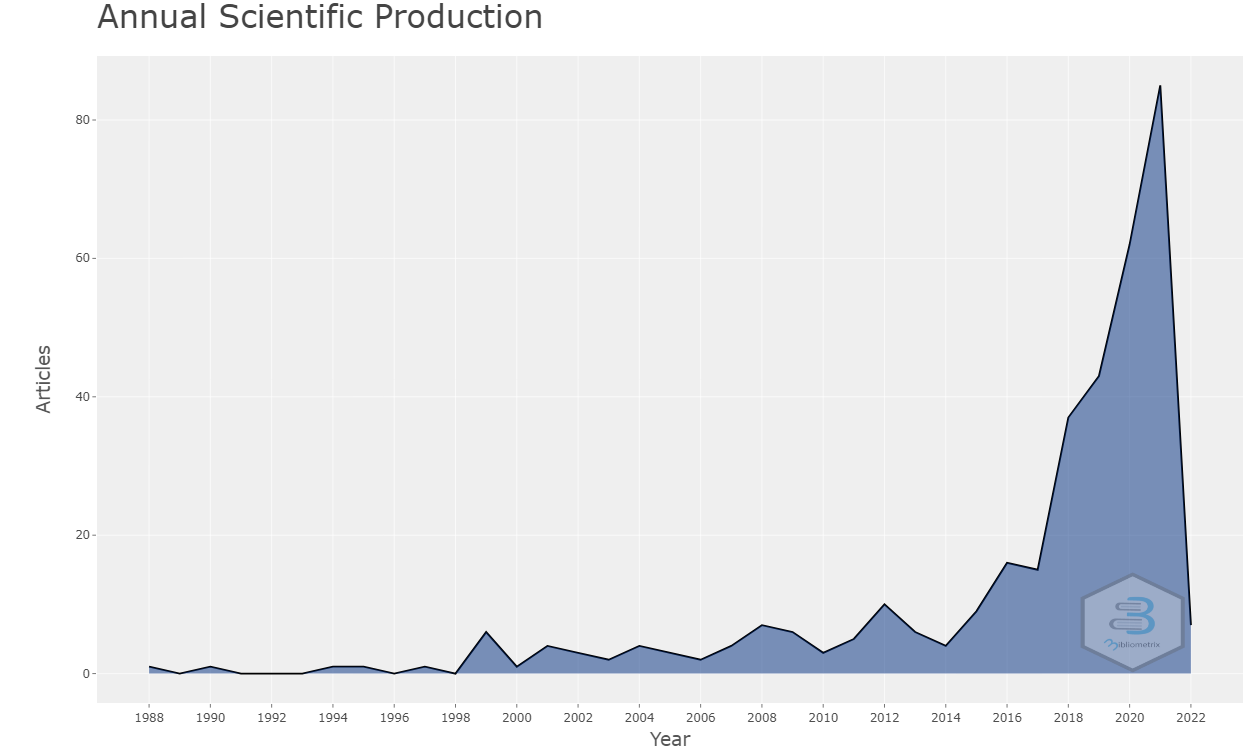
\includegraphics[width=1\textwidth]{experiments/KawaiiStheno/PesqBibliogr/NeurocienciaIIA/WoS-20220206/scientificProdution.png}
    \caption{Evolução da produção científica no \dataset\   kawaiistheno.}
    \label{fig:evol:anual:kawaiistheno}
\end{figure}

Observando a figura \ref{fig:evol:anual:kawaiistheno}, podemos perceber uma evolução gradativa na quantidade de artigos ao longo dos anos, tendo uma explosão de novos artigos a partir do ano de 2014.

\subsection{Evolução das Citações}

\begin{figure}
    \centering
    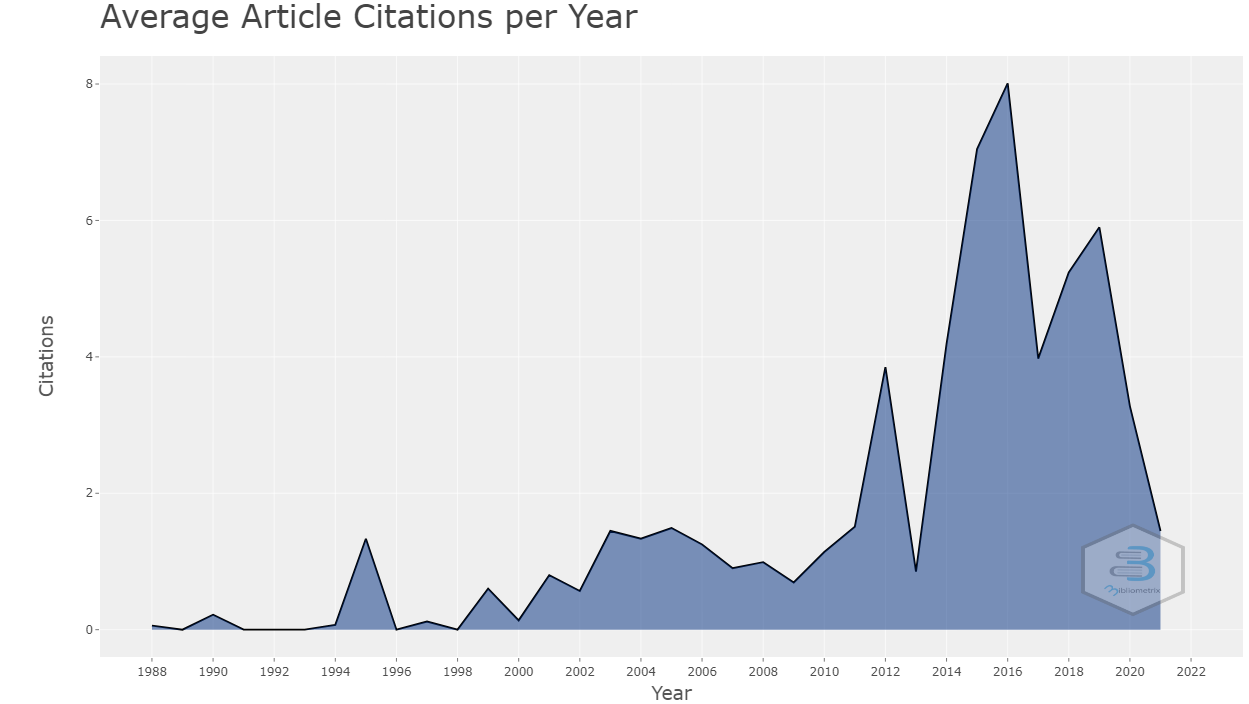
\includegraphics[width=1\textwidth]{experiments/KawaiiStheno/PesqBibliogr/NeurocienciaIIA/WoS-20220206/citationsYear.png}
    \caption{Evolução das citações ao \dataset\   kawaiistheno.}
    \label{fig:cit:anual:kawaiistheno}
\end{figure}

É possível observar em \ref{fig:evol:anual:kawaiistheno} que o número de citações começou a crescer lentamente a partir de 1998, sofrendo uma explosão neste crescimento em 2014. Se compararmos com a figura \ref{fig:evol:anual:kawaiistheno} podemos perceber que neste ano, a produção científica também teve um aumento considerável de artigos produzidos, indicando que 2014 foi um ano de expre

\subsection{Three-Field Plots (Sankey diagram)}